\chapter{Bộ dữ liệu và khảo sát dữ liệu}
\section{Nguồn gốc và khả năng sử dụng}
Bộ \dataset{} do Stephan Matzka công bố trên UCI Machine Learning Repository với DOI \url{10.24432/C5HS5C}, giấy phép CC BY 4.0 \cite{uci2020,matzka2020}. Tác giả xây dựng dữ liệu tổng hợp nhằm phản ánh một số tình huống bảo trì dự đoán. Đây là thuận lợi cho bài tập có thể chia sẻ công khai, đồng thời phải được nêu rõ khi diễn giải kết quả. Tệp CSV mà pipeline sử dụng có SHA-256 \src{dc6630cd9b1f0f853922fad78a1b6436570d3f1ec863f1dd5c4340ac56bc8a8e}. Hàm tải của dự án xác thực nguồn trước khi sử dụng, giúp phát hiện nếu nội dung tệp thay đổi ngoài dự kiến.

\section{Cấu trúc trường dữ liệu}
Tệp thực tế có 14 cột. \src{UDI} là số định danh dòng và \src{Product ID} là mã sản phẩm. \src{Type} nhận một trong ba giá trị L, M, H. Năm phép đo gồm nhiệt độ không khí, nhiệt độ quá trình, tốc độ quay, mô-men xoắn và thời gian hao mòn dụng cụ. \src{Machine failure} là nhãn tổng thể. Năm cột TWF, HDF, PWF, OSF và RNF mô tả chế độ hỏng. Tên \src{UDI} được ghi theo chính tệp CSV tải về; trang giới thiệu bộ dữ liệu dùng cách đặt tên có thể khác. Báo cáo ưu tiên schema của hiện vật thực nghiệm.

\begin{table}[H]\centering\caption{Các trường được đưa vào mô hình}\label{tab:features}
\begin{tabularx}{\textwidth}{p{4.8cm}p{2.5cm}X}\toprule
Trường & Kiểu & Ý nghĩa và xử lý\\\midrule
Type & Phân loại & Mã loại sản phẩm L/M/H; one-hot encoding\\
Air temperature [K] & Số thực & Nhiệt độ không khí; chuẩn hóa trên train\\
Process temperature [K] & Số thực & Nhiệt độ quá trình; chuẩn hóa trên train\\
Rotational speed [rpm] & Số nguyên & Tốc độ quay; chuẩn hóa trên train\\
Torque [Nm] & Số thực & Mô-men xoắn; chuẩn hóa trên train\\
Tool wear [min] & Số nguyên & Thời gian hao mòn; chuẩn hóa trên train\\\bottomrule
\end{tabularx}
\end{table}
Việc loại trừ các cột nguyên nhân hỏng là quyết định thiết kế quan trọng hơn việc thử thêm thuật toán. Chúng là các chỉ báo lỗi đã xác định, không phải thông số cảm biến độc lập trước quyết định. Nếu dùng chúng để dự báo \src{Machine failure}, bài toán huấn luyện sẽ khác hợp đồng API có sáu trường. Danh sách cho phép trong \src{features.py} khiến mã dừng ngay khi thiếu trường bắt buộc, nhãn không nhị phân hoặc loại sản phẩm không hợp lệ.

\section{Quy mô, cân bằng lớp và giá trị thiếu}
Tập có 10.000 dòng, không có giá trị thiếu trong 14 cột. Có 9.661 bản ghi không hỏng và 339 bản ghi hỏng, tương ứng tỷ lệ dương 3,39\%. Hình~\ref{fig:class} cho thấy chênh lệch đáng kể giữa hai lớp. Một số đo chỉ dựa trên số dự đoán đúng sẽ bị lớp đông chi phối, vì vậy báo cáo ưu tiên AP và các chỉ số từ ma trận nhầm lẫn.

\begin{figure}[H]\centering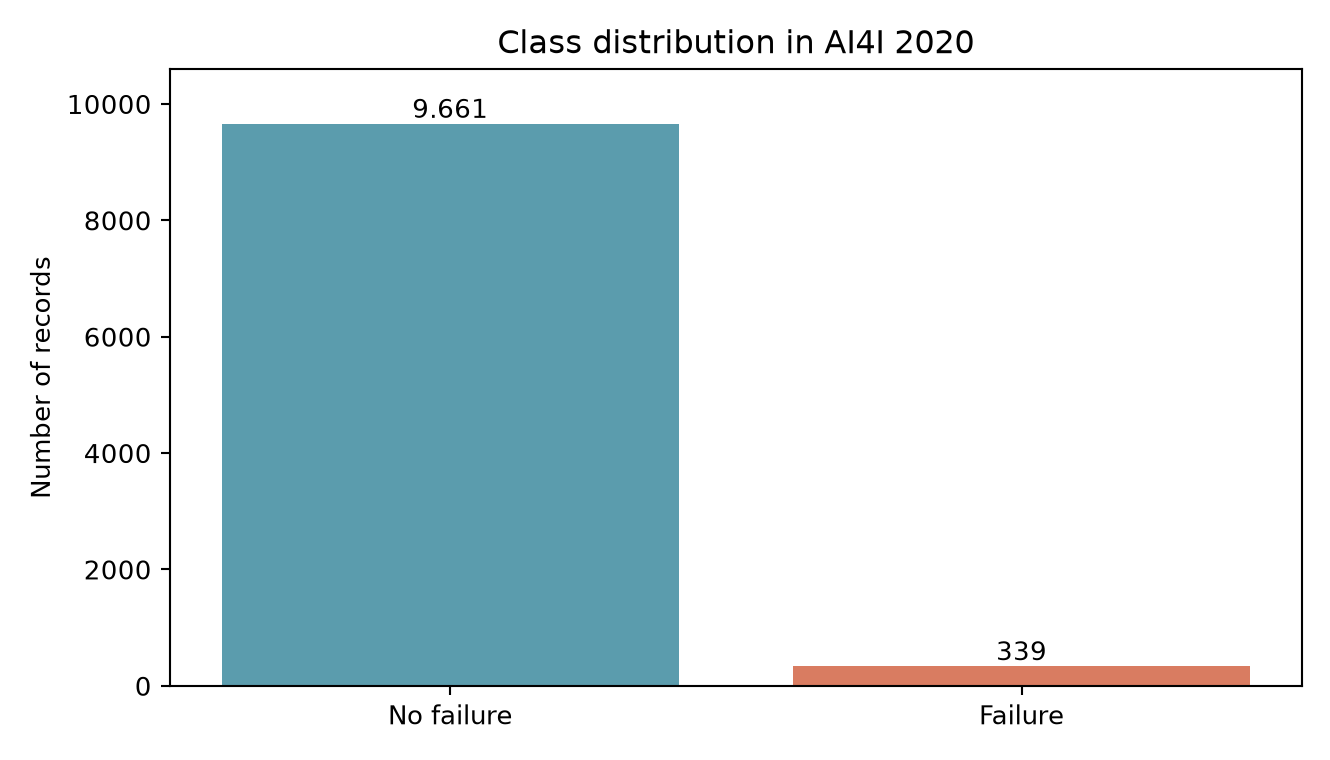
\includegraphics[width=.78\textwidth]{class_balance.png}\caption{Phân bố nhãn trong dữ liệu gốc. Nguồn: tính từ CSV đã xác thực SHA-256.}\label{fig:class}\end{figure}

\begin{table}[H]\centering\caption{Số lượng và tỷ lệ hỏng theo loại sản phẩm}\label{tab:type}
\begin{tabular}{lrrr}\toprule Loại & Số bản ghi & Số hỏng & Tỷ lệ hỏng\\\midrule
L & 6.000 & 235 & 3,92\% \\
M & 2.997 & 83 & 2,77\% \\
H & 1.003 & 21 & 2,09\% \\
\bottomrule

\end{tabular}\end{table}
Ba loại sản phẩm không có cùng số quan sát: L có 6.000, M có 2.997 và H có 1.003. Tỷ lệ lỗi theo nhóm trong Bảng~\ref{tab:type} là mô tả của dữ liệu, không chứng minh rằng một loại sản phẩm gây hỏng. Muốn kết luận nhân quả cần hiểu cơ chế sinh dữ liệu và kiểm soát các biến khác. Trong phục vụ mô hình, giá trị \src{Type} ngoài L/M/H bị API từ chối; bộ mã hóa vẫn cấu hình \src{handle_unknown="ignore"} để pipeline có hành vi xác định nếu được dùng trong ngữ cảnh khác.

\begin{figure}[H]\centering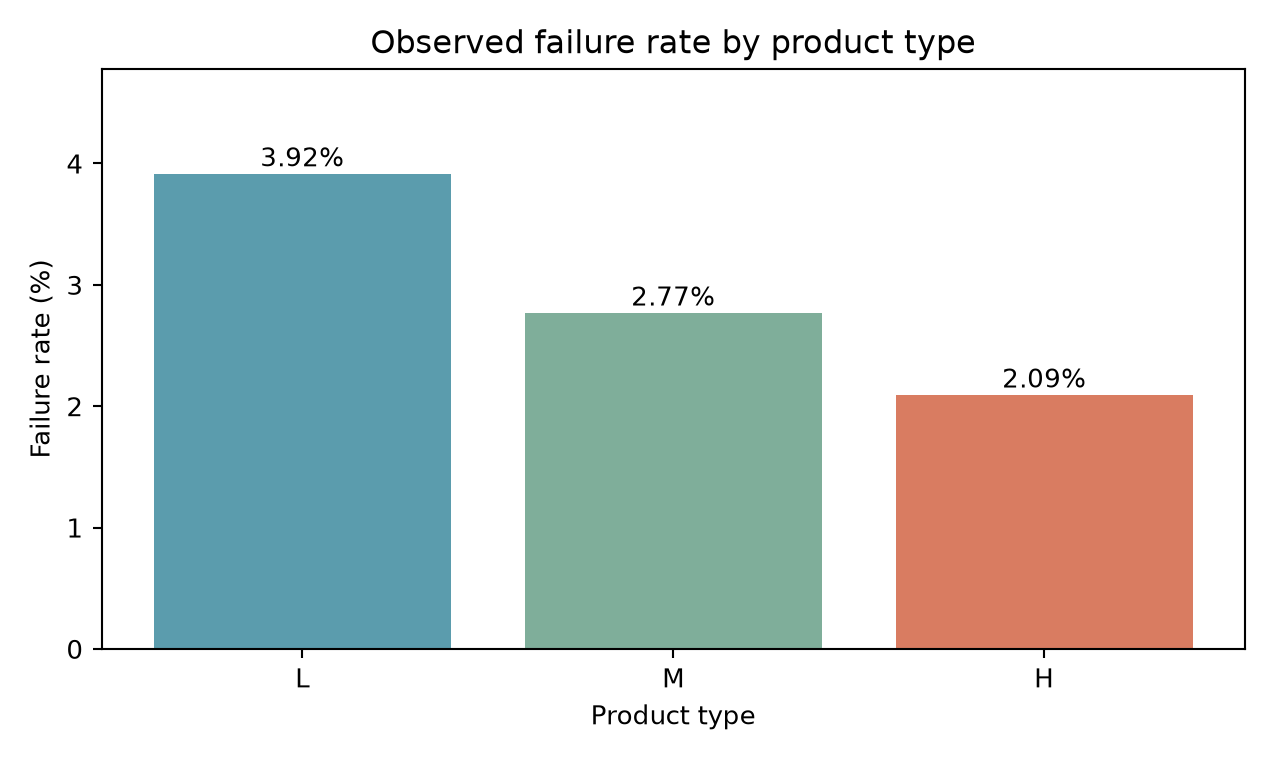
\includegraphics[width=.98\textwidth]{type_failure_rate.png}\caption{Quy mô và tỷ lệ bản ghi hỏng theo loại sản phẩm.}\label{fig:type}\end{figure}

\section{Phân phối cảm biến và chế độ hỏng}
Hình~\ref{fig:sensors} đặt cạnh phân phối của năm biến số theo nhãn. Các biểu đồ giúp nhìn vùng giá trị chồng lấn và những khác biệt dễ thấy; chúng không thể hiện quan hệ có điều kiện giữa các biến. Từ tệp dữ liệu, trung bình mô-men xoắn của nhóm hỏng là 50,17 Nm so với 39,63 Nm của nhóm không hỏng; hao mòn trung bình lần lượt là 143,78 và 106,69 phút. Nhiệt độ không khí trung bình là 300,89 K ở nhóm hỏng và 299,97 K ở nhóm bình thường. Những con số này mô tả tương quan biên và không xác định một quy tắc chẩn đoán đơn lẻ.

\begin{figure}[H]\centering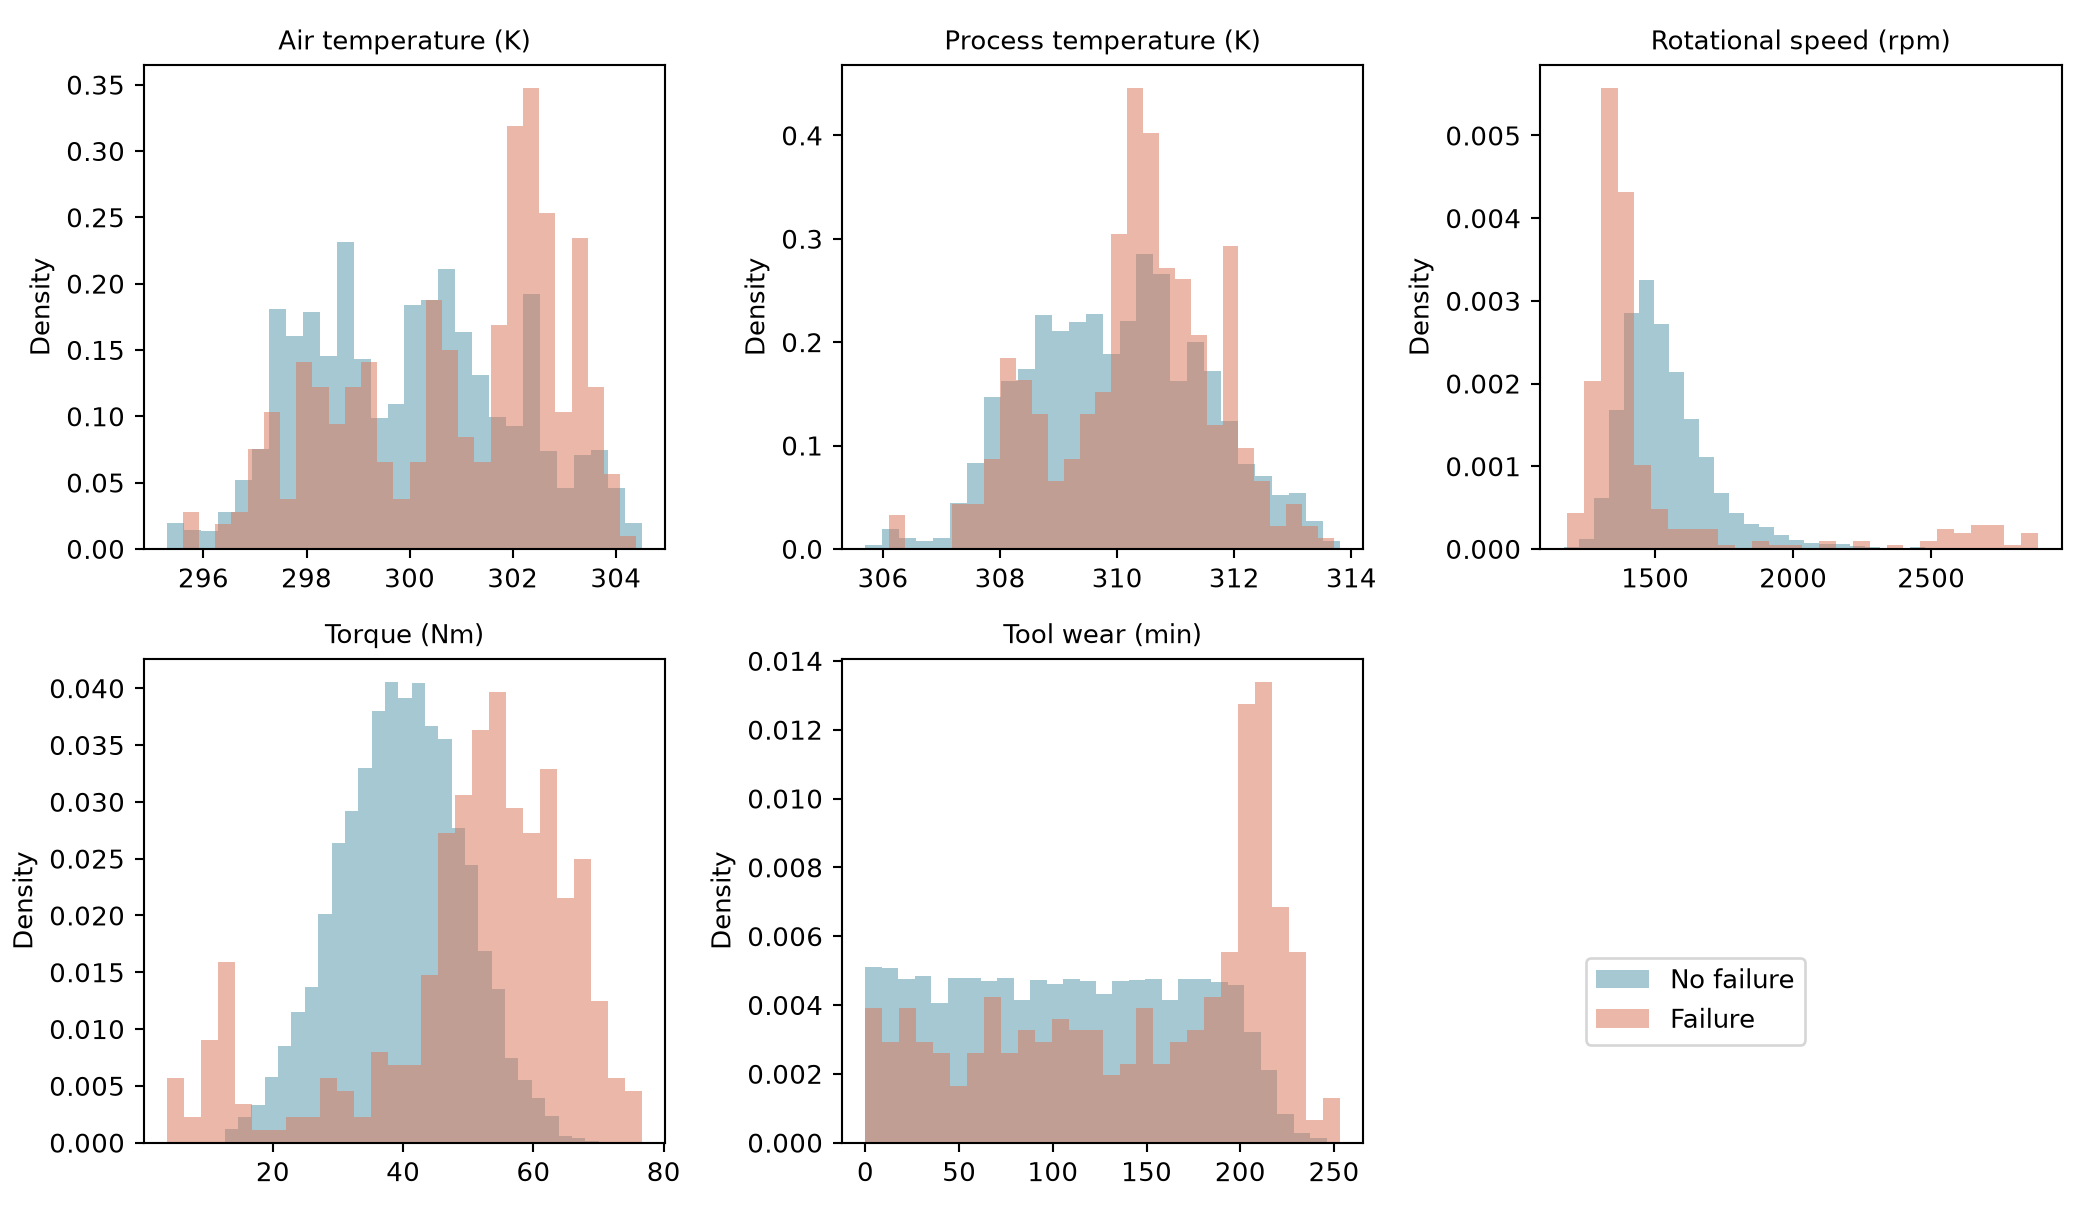
\includegraphics[width=.98\textwidth]{sensor_distributions.png}\caption{Phân phối các phép đo theo nhãn, dùng để khảo sát trước mô hình hóa.}\label{fig:sensors}\end{figure}

Các cột chế độ hỏng có số dương lần lượt là TWF 46, HDF 115, PWF 95, OSF 98 và RNF 19. Tổng các số này không nhất thiết bằng 339 do một bản ghi có thể thuộc nhiều chế độ. Chúng chỉ được dùng để mô tả bộ dữ liệu; mô hình không nhận chúng làm đầu vào. Việc giữ ranh giới này cũng làm cho đánh giá ngoại tuyến nhất quán với sáu trường mà API nhận.

\begin{figure}[H]\centering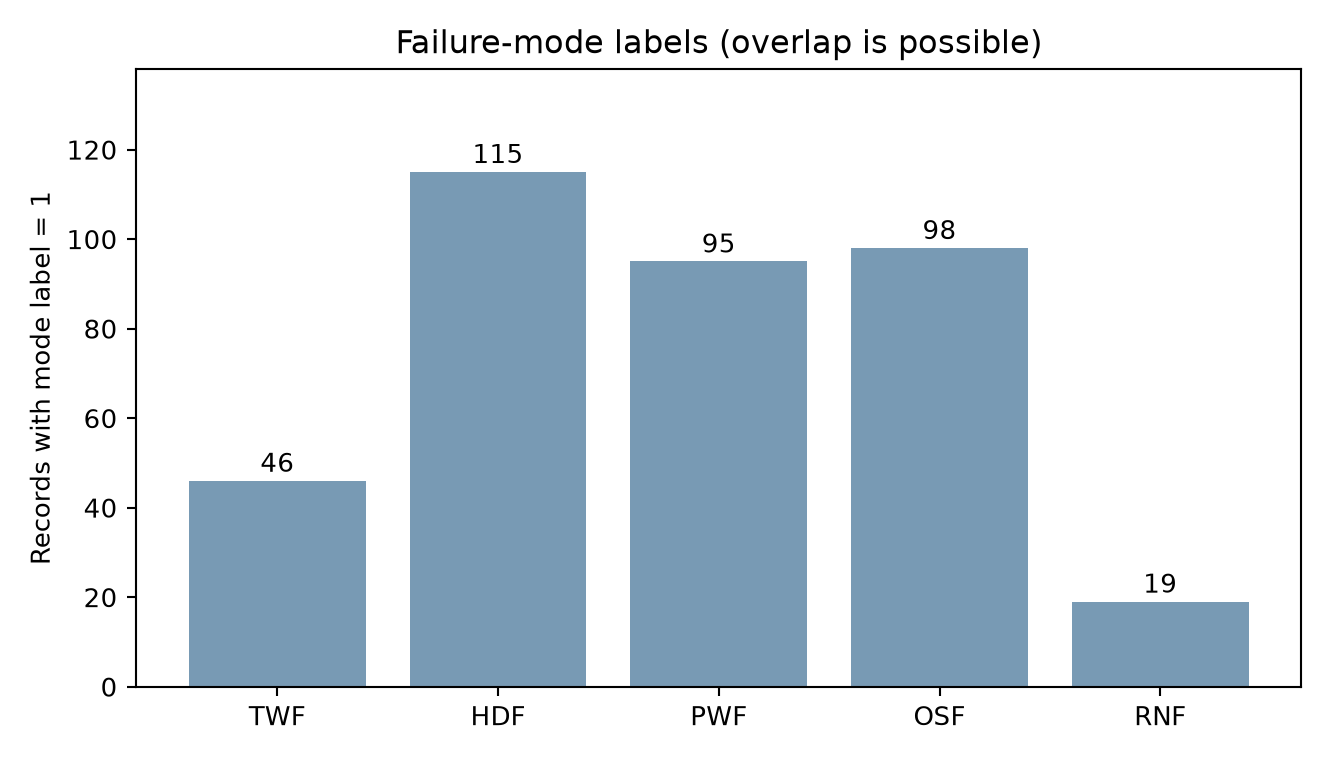
\includegraphics[width=.82\textwidth]{failure_modes.png}\caption{Số bản ghi dương theo từng cột chế độ hỏng; các nhóm có thể chồng lấn.}\label{fig:modes}\end{figure}

\section{Thiết kế phép chia tập}
Đầu tiên nhóm tách 20\% bản ghi làm test, có phân tầng theo nhãn. Sau đó lấy 20\% của phần 80\% còn lại làm validation. Kết quả là tỷ lệ 64/16/20, seed 42. Bảng~\ref{tab:split} cho thấy tỷ lệ hỏng được duy trì gần như nhau. Test được giữ riêng cho đến khi chọn xong mô hình và ngưỡng.

\begin{table}[H]\centering\caption{Phân chia dữ liệu dùng trong thực nghiệm}\label{tab:split}
\begin{tabular}{lrrr}\toprule Tập & Số bản ghi & Số hỏng & Tỷ lệ hỏng\\\midrule
Train & 6.400 & 217 & 3,39\% \\
Validation & 1.600 & 54 & 3,38\% \\
Test & 2.000 & 68 & 3,40\% \\
\bottomrule

\end{tabular}\end{table}

Không có khóa thiết bị lặp lại để thực hiện chia theo máy, và không có chuỗi thời gian để chia theo mốc. Do đó đánh giá này là nội bộ trên tập tĩnh. Nếu có dữ liệu thực tế, thiết kế phù hợp hơn sẽ tách theo thiết bị hoặc theo thời gian triển khai, tránh để những trạng thái rất gần nhau của một máy xuất hiện cả ở train và test. Cần xác định rõ ``thời điểm dự báo'' và khoảng thời gian trước hỏng trước khi gọi kết quả là cảnh báo sớm.

